\documentclass[letterpaper,11pt]{article}

\usepackage{latexsym}
\usepackage[empty]{fullpage}
\usepackage{titlesec}
\usepackage{marvosym}
\usepackage[usenames,dvipsnames]{color}
\usepackage{verbatim}
\usepackage{enumitem}
\usepackage[hidelinks]{hyperref}
\usepackage{fancyhdr}
\usepackage[english]{babel}
\usepackage{tabularx}
\usepackage{fontawesome5}
\usepackage{multicol}
\setlength{\multicolsep}{-3.0pt}
\setlength{\columnsep}{-1pt}
\input{glyphtounicode}

%new packages

\usepackage{fontenc}
\usepackage{amsmath}
\usepackage{amssymb}
\usepackage{graphicx}



%----------FONT OPTIONS----------

\pagestyle{fancy}
\fancyhf{} % clear all header and footer fields
\fancyfoot{}
\renewcommand{\headrulewidth}{0pt}
\renewcommand{\footrulewidth}{0pt}

% Adjust margins
\addtolength{\oddsidemargin}{-0.6in}
\addtolength{\evensidemargin}{-0.5in}
\addtolength{\textwidth}{1.19in}
\addtolength{\topmargin}{-.7in}
\addtolength{\textheight}{1.4in}

\urlstyle{same}

\raggedbottom
\raggedright
\setlength{\tabcolsep}{0in}

% Sections formatting
\titleformat{\section}{
  \vspace{-4pt}\scshape\raggedright\large\bfseries
}{}{0em}{}[\color{black}\titlerule \vspace{-5pt}]



% Ensure that generate pdf is machine readable/ATS parsable
\pdfgentounicode=1

%-------------------------
% Custom commands
\newcommand{\resumeItem}[1]{
  \item\small{
    {#1 \vspace{-2pt}}
  }
}

\newcommand{\classesList}[4]{
    \item\small{
        {#1 #2 #3 #4 \vspace{-2pt}}
  }
}

\newcommand{\resumeSubheading}[4]{
  \vspace{-2pt}\item
    \begin{tabular*}{1.0\textwidth}[t]{l@{\extracolsep{\fill}}r}
      \textbf{#1} & \textbf{\small #2} \\
      \textit{\small#3} & \textit{\small #4} \\
    \end{tabular*}\vspace{-7pt}
}

\newcommand{\resumeSubSubheading}[2]{
    \item
    \begin{tabular*}{0.97\textwidth}{l@{\extracolsep{\fill}}r}
      \textit{\small#1} & \textit{\small #2} \\
    \end{tabular*}\vspace{-7pt}
}

\newcommand{\resumeProjectHeading}[2]{
    \item
    \begin{tabular*}{1.001\textwidth}{l@{\extracolsep{\fill}}r}
      \small#1 & \textbf{\small #2}\\
    \end{tabular*}\vspace{-7pt}
}


\newcommand{\resumeSubItem}[1]{\resumeItem{#1}\vspace{-4pt}}

\renewcommand\labelitemi{$\vcenter{\hbox{\tiny$\bullet$}}$}
\renewcommand\labelitemii{$\vcenter{\hbox{\tiny$\bullet$}}$}

\newcommand{\resumeSubHeadingListStart}{\begin{itemize}[leftmargin=0.0in, label={}]}
\newcommand{\resumeSubHeadingListEnd}{\end{itemize}}
\newcommand{\resumeItemListStart}{\begin{itemize}}
\newcommand{\resumeItemListEnd}{\end{itemize}\vspace{-5pt}}

\begin{document}
\fontfamily{cmr}\selectfont
\begin{center}
\parbox{3.0cm}{%
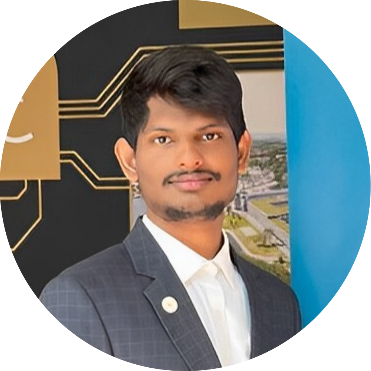
\includegraphics[width=2.7cm,clip]{images/resume_pic_m.png}}
}
\parbox{\dimexpr\linewidth-3.8cm\relax}{
\vspace{-20pt}
\begin{tabularx}{\linewidth}{L r} \\
    {\Huge \scshape  Venkata Sai Yakkshit Reddy Asodi}~
    \href{https://www.cedzlabs.com/yakkshit}{\vspace{1pt}}\\
      Berlin, Germany. \\ \vspace{1pt}
     \small \raisebox{-0.1\height}\faPhone\ +91 8179936156 ~ \href{mailto:saiyakkshit2001@gmail.com}{\raisebox{-0.2\height}\faEnvelope\  {saiyakkshit2001@gmail.com}} ~ 
    \href{https://linkedin.com/in/yakkshit/}{\raisebox{-0.2\height}\faLinkedin\ {yakkshit}}  ~
    \href{https://yakkshit.com/}{\raisebox{-0.2\height}\faGlobe\ {yakkshit.com}}  ~
    \href{https://github.com/yakkshit}{\raisebox{-0.2\height}\faGithub{ yakkshit}}
    \vspace{-8pt}
\end{tabularx}
}
\end{center}

\vspace{-23pt}
%-----------SUMMARY-----------
\section{Summary}
Aspiring Software Engineer with a passion for problem-solving and building scalable software solutions. Eager to gain hands-on experience through internships to further refine software development skills. Proficient in JavaScript, Python, and familiar with system design, algorithm development, and debugging. Thrives in collaborative and fast-paced environments, eager to apply knowledge to real-world challenges.

%-----------TECHNICAL SKILLS-----------
\section{Technical Skills}
\begin{itemize}[leftmargin=0.15in, label={}]
\small{
\item \textbf{Programming Languages:} Java, C++, Python, JavaScript.
\item \textbf{Web Technologies:} HTML5, CSS3, React, Next.js, TailwindCSS.
\item \textbf{Databases:} MySQL, MongoDB, Supabase.
\item \textbf{Tools:} Git, Docker, Postman, Swagger.
\item \textbf{Cloud:} AWS, Azure.
\item \textbf{Version Control:} Git, GitHub, GitLab.
\item \textbf{Methodologies:} Agile (Scrum, Kanban).
}
\end{itemize}

%-----------EXPERIENCE-----------
\section{Experience}

\resumeSubHeadingListStart
\resumeSubheading
{\large Circleup AG \faBuilding}{January 2024 -- Present}
  {Lead Full Stack Engineer (Frontend Focus)}{\faMapMarker \hspace{0.1cm} Zurich, Switzerland}\\
\vspace{10pt}
\textbf{Responsibilities:}
\resumeItemListStart
\vspace{-10pt}
\resumeItem{Led development of scalable, responsive web applications using React and Django. Focused on user-centered design and seamless integration of APIs for LLM automation.}
\resumeItem{Enhanced application performance, reliability, and UI/UX using testing frameworks and best practices.}
\resumeItem{Collaborated in Agile sprints to ensure project delivery and application quality.}
\resumeItemListEnd
\vspace{-3pt}

\resumeSubheading
{Cedzlabs \faBuilding}{March 2023 -- December 2023}
{Full Stack Developer (Frontend Focus)}{\faMapMarker \hspace{0.1cm} India}\\
\vspace{10pt}
\textbf{Responsibilities:}
\vspace{-10pt}
\resumeItemListStart
\resumeItem{Developed interactive user interfaces for event scheduling platforms using React and Next.js, optimizing for accessibility and cross-platform performance.}
\resumeItem{Collaborated with backend teams to integrate APIs and ensure seamless user interaction in cloud environments using Firebase and Supabase.}
\resumeItemListEnd
\vspace{-3pt}

%-----------PROJECTS-----------
\section{Projects}

\resumeProjectHeading
{\textbf{AI Resume Generator} $|$ \emph{Next.js, TailwindCSS, Azure}}{August 2023}\\
\vspace{6pt}
\textbf{Description:}
\vspace{-5pt}
\resumeItemListStart
\resumeItem{Built an AI-powered resume generator using Next.js, TailwindCSS, and Azure Cloud. The system uses AI to generate tailored resumes based on job descriptions and user input, integrated with cloud services for scalability.}
\resumeItemListEnd

\resumeProjectHeading
{\textbf{Currency Converter App} $|$ \emph{React, Mapbox API, REST}}{April 2023}\\
\vspace{6pt}
\textbf{Description:}
\vspace{-5pt}
\resumeItemListStart
\resumeItem{Developed a real-time currency conversion app, integrating Mapbox API for geographic data visualization. Utilized REST APIs to fetch and display exchange rates dynamically.}
\resumeItemListEnd

%-----------ACHIEVEMENTS-----------
\section{Achievements}
\begin{itemize}
\item Microsoft Hackathon 2023 Winner – Developed an AI Resume Tuner using RAG and multimodal LLMs.
\item Contributed to open-source projects, including a popular React UI library.
\item Active participant in tech meetups, hackathons, and coding challenges.
\end{itemize}

\vspace{10pt}
\end{document}